\TUchapter{ECM Replay Software}

This chapter discusses the specific implementation of the method outlined in the previous chapter.

\TUsection{Recording an extraction}

The first step in extracting data from an ECM was to determine how the manufacturers themselves extracted
the desired data. Without performing extensive static or dynamic analysis of the internals of the maintenance
software, it was determined that the best way to determine the extraction process was to record the messages
sent by the maintenance software to the ECM. Recording these messages could take place at two information boundaries,
the network or the diagnostic link connector driver.

\TUsubsection{Network Recording}

Communication between the ECM and the maintenance software may be recorded at the network level, but this method
has some drawbacks.

First, recording traffic from the network requires additional hardware. In addition to the hardware normally required
to connect to ECMs, network recording requires some means of physically connecting to the network. In addition to the 
connection apparatus, network-logging device is also required. As it is not uncommon for ECM communications to take place over both J1708 and J1939, 
this hardware must be able to record both protocols.

Secondly, some meaning is lost. Applications typically use RP1210\_SendCommand calls to filter out broadcast communications
or other irrelevant messsages. Observation strictly at the network level does not provide any clues as to which messages
the application might be filtering, so unimportant messages must be identified and filtered out.

\TUsubsection{RP1210 Recording}

An alternate method of recording information extraction is to record calls made to the RP1210 drivers
by the maintenance software. This has the advantage of not requiring additional hardware to 
record network traffic, and to abstract away the details of transport-layer operations of J1939. It does however
still require a Diagnostic Link Connector.

Recording calls made to these RP1210 drivers was accomplished using a technique called API hooking\cite{Berdajs2010}.
A custom lightweight debugger was written using the PyDBG tool\cite{Amini2012}. Upon attaching the debugger to the software
in question, the debugger searches process memory for any loaded RP1210 drivers. Upon discovering a loaded RP1210
driver module, it places breakpoints on the following RP1210 function addresses:

\begin{enumerate}
  \item RP1210\_ReadMessage
  \item RP1210\_SendMessage
  \item RP1210\_ClientConnect
  \item RP1210\_SendCommand
  \item RP1210\_ClientDisconnect
\end{enumerate}

This is a proper subset of the functions that the RP1210 standard requires that drivers implement, covering the functions that
are used for setting up the ECM communications session and actually extracting the data.
When execution hits one of these breakpoints, the debugger reads all arguments passed to the function when it was called,
and places a breakpoint on the function's return address so that return values can be read as well. In this way, all
messages sent to and received from the ECM are recorded by the debugging software.

This approach has an advantage in that it doesn't require any additional hardware. Since the price of 
commercial vehicle network loggers can reach several hundred to several thousand dollars, cost-effectiveness should
not be overlooked. It also shows exactly which messages the application receives, which aids in determining which
messages are important. API hooking code is included in Appendix \ref{app:trace}.

\begin{figure}[h]
  \centering
  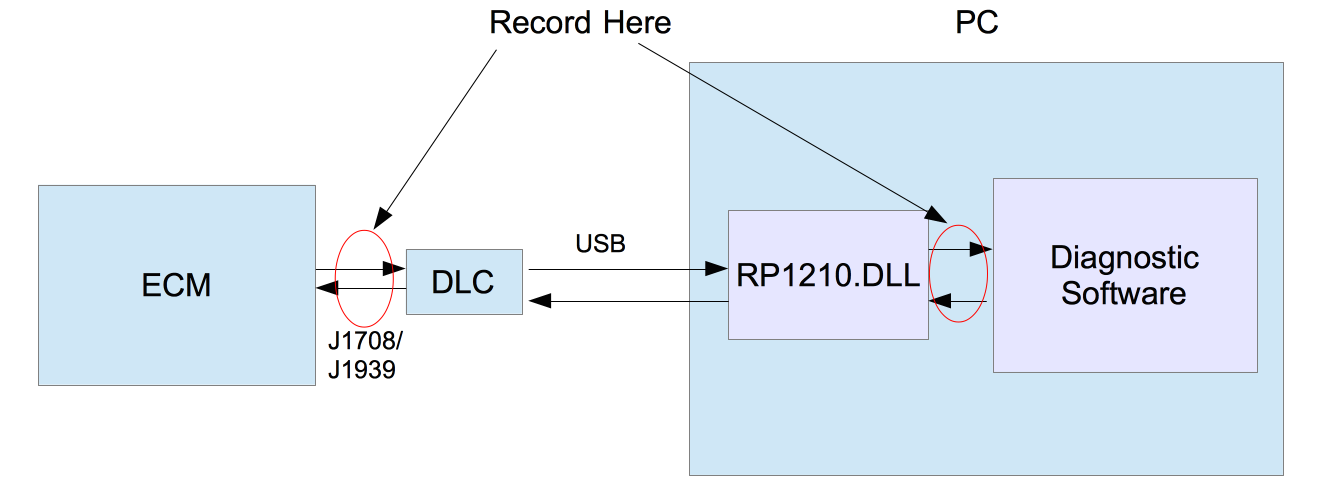
\includegraphics[scale=0.5]{RecordPoint}
  \caption{Information Boundaries for Recording}
  \label{fig:infoboundaries}
\end{figure}

\TUsection{Replaying an Extraction}

In order to ensure that the method of evidence extraction was as general as possible, evidence extraction was implemented
by simply replaying requests recorded during an actual information extraction. In the case of encrypted requests, where
the same request may be encrypted differently depending upon details of individual sessions, a transformation function
to decrypt the message and store it in a plaintext format needs to be specified. As each manufacturer's protocols
are proprietary, different transformation functions must be defined for different manufacturers' products.

After each request is replayed, responses to that request are recorded. The extraction data are stored as a list of 
key-value pairs, where the key is the request (transformed to a plaintext format, if applicable) and the value is
a list of all messages that the ECM sends in response to that request. This list is then serialized into a format
that can be stored in a file on disk; this file is the logical equivalent of a hard disk image.

As it has been observed that requests sent to the ECM may alter the state of the ECM, the replay mechanism must
be designed so that this is taken into account. The stored replay data are treated as a circular queue, with a current
index maintained during the extraction. Upon receipt of a message, the index is advanced until a matching response is found.
If responses to requests depend on earlier messages, receipt of the earlier messages will advance the index to
the expected response.

\TUsubsection{Replaying Extracted Data}

Just as a transformation function may need to be specified for extraction of encrypted information, such a transformation
function may also need to be specified during replay. A comparison function needs to be specified, as the message format may
preclude the use of straight comparison of request data.

The solution arrived at uses two separate threads of control, one handling J1708/1587 communications and the other
handling J1939 communications. Each has its own protocol-specific response queue, though the two queues are both
stored in the same file for evidence storage and encryption.


